\section{Joint inversion}\label{sec:joint}
The term joint inversion denotes the simultaneous inversion of a number of different data types.
We can classify different types according to the relation of the associated parameters:
\begin{enumerate}
	\item Identical parameters is historical the classical joint inversion, e.g. both DC and EM aim at $\rho$.
	\item Parameters are indirectly connected by petrophysical relations, e.g. ERT and GPR both aiming at water content.
	\item Independent parameters. In this case only the structures can be linked to each other. For simple models this can involve the inversion of the geometry. For fixed models structural information is exchanged\footnote{Note that this type is formally a structurally coupled cooperative inversion.}.
\end{enumerate}

%%%%%%%%%%%%%%%%%%%%%%%%%%%%%%%%%%%%%%%%%%%%%%%%%%%%%%%%%%%%%%%%%%%%%%%%%%%
\subsection{Classical joint inversion of DC and EM soundings}\label{sec:jointdcem}
File \file{doc/tutorial/code/joint/dcem1dinv.cpp}\\
First, let us consider to jointly invert different electromagnetic methods, e.g. direct current (DC) and Frequency Domain Electromagnetic (FDEM).
For the latter we assume a two-coil system in horizontal coplanar model with 10 frequencies between 110\,Hz and 56\,kHz.
Whereas DC resistivity yields apparent resistivities, the FDEM data are expressed as ratio between secondary and primary field in per cent.

The two ready methods \lstinline|DC1dModelling| and \lstinline|FDEM1dModelling| are very easily combined since they use the same block model.
In the response function the two vectors are combined.
We create a new modelling class that derives from the base modelling class\footnote{In order to use the classes, \file{dc1dmodelling.h} and \file{em1dmodelling.h} have to be included.} and has two members of the individual classes, which must be initialized in the constructor.
Alternatively we could derive from one of the two classes and use only a member of the other.

\begin{lstlisting}[language=C++,morekeywords={RVector,RMatrix}]
class DCEM1dModelling : public ModellingBase {
public:
    DCEM1dModelling( size_t nlay, RVector & ab2, RVector & mn2, 
                     RVector & freq, double coilspacing, bool verbose ) : 
    	ModellingBase( verbose ), // base constructor
    	fDC_( nlay, ab2, mn2, verbose ), // FDEM constructor
    	fEM_( nlay, freq, coilspacing, verbose ) { // DC constructor 
          setMesh( createMesh1DBlock( nlay ) ); // create mesh
    }
    RVector response( const RVector & model ){ // paste together responses
        return cat( fDC_.response( model ), fEM_.response( model ) ); 
    }
protected:
    DC1dModelling fDC_;
    FDEM1dModelling fEM_;
};
\end{lstlisting}

In the response function both response functions are called and combined using the cat command.
We set the usual transformation (log for apparent resistivity and logLU for the resistivity) and inversion (Marquardt scheme) options as above.
In case of identical responses (e.g. apparent resistivities) this would be the whole thing.
Here we have to care about the different data types (cf. section \ref{sec:mt1d}), i.e. always positive, log-distributed $\rho_a$ from DC and possibly negative, linearly distributed, relative magnetic fields.
The transformations are again combined using \lstinline|CumulativeTrans|
\begin{lstlisting}[language=C++,morekeywords={RVector,RMatrix}]
    RTransLog transRhoa;
    RTrans transEM;
    CumulativeTrans< RVector > transData;
    transData.push_back( transRhoa, ab2.size() );
    transData.push_back( transEM, freq.size() * 2 );
\end{lstlisting}

In the code we create a synthetic model \lstinline|synthModel|, calculate the forward response and noisify it by given noise levels.

\begin{lstlisting}[language=C++,morekeywords={RVector,RMatrix}]
    /*! compute synthetic model (created before) by calling f */
    RVector synthData( f( synthModel ) );   
    /*! error models: relative percentage for DC, absolute for EM */
    RVector errorDC = synthData( 0, ab2.size() ) * errDC / 100.0;
    RVector errorEM( freq.size() * 2, errEM );
    RVector errorAbs( cat( errorDC, errorEM ) );    
    /*! noisify synthetic data using the determined error model */
    RVector rand( synthData.size() );
    randn( rand );
    synthData = synthData + rand * errorAbs;
\end{lstlisting}

The inversion is converging to a $\chi^2$ value of about 1, i.e. we fit the data within error bounds.
Finally a resolution analysis is done to determine how well the individual parameters (2 thickness and 3 resistivitiy values) are determined.
We can compare it with single inversions by drastically increasing the error level for one of the methods by a factor of 10.
Table \ref{tab:dcemresolution} shows the resulting diagonal values of the resolution matrix for a three-layer model.
The first layer is well resolved in all variants except the first layer resistivity for EM.
Considering the values for the other resistivities we can clearly see that EM is detecting the good conductor and DC describes the resistor as expected from the theory.

\begin{table}[h]%
\centering
\begin{tabular}{r|ccccc}
Method & $d_1$=20\,m & $d_2$=20\,m & $\rho_1$=200\,$\Omega$m & $\rho_2$=10\,$\Omega$m & $\rho_3$=50\,$\Omega$m \\ \hline
Joint inversion: & 0.98 & 0.46 & 0.98 & 0.67 & 0.57 \\
EM dominated:    & 0.97 & 0.36 & 0.71 & 0.66 & 0.20 \\
DC dominated:    & 0.96 & 0.21 & 0.97 & 0.32 & 0.62  
\end{tabular}
\caption{Resolution measures for Joint inversion and quasi-single inversions using an error model increased by a factor of 10.}\label{tab:dcemresolution}
\end{table}

%%%%%%%%%%%%%%%%%%%%%%%%%%%%%%%%%%%%%%%%%%%%%%%%%%%%%%%%%%%%%%%%%%%%%%%%%%%
\subsection{Block joint inversion of DC/MRS data}\label{sec:blockjoint}
%File \file{doc/tutorial/code/joint/dc\_mt\_block1d.cpp}\\
If the underlying parameters of the jointed inversion are independent, a combination can only be achieved via the geometry.
For the case of a block 1d discretization both methods are affected by the layer thicknesses.
%We use the same methods as before \sperre

Similar to the above example, we create a combined modelling class that is derived from one method, in this case \lstinline|MRS1DBlockModelling|.
This one is a block model (water content and thickness) variant of the magnetic resonance sounding (MRS) modelling \lstinline|MRSModelling|.
The class has a DC resistivity forward modelling and holds the number of layers \lstinline|nlay|.

The model is created in the constructor using \lstinline|createMesh1DBlock( nlay, 2 )| that is able to hold, additionally to the thickness (region 0), multiple properties, here water content (region 1) and resistivity (region 2).
From the model vector the thickness, water content (or their combination) and resistivity has to be extracted and the result of the two forward calls are combined using the cat command.
The Jacobian is by default brute force, which is quite cheap for block models.

\begin{lstlisting}[language=C++,morekeywords={RVector,RMatrix}]
class DC_MRS_BlockModelling : public MRS1dBlockModelling{
public:
    DC_MRS_BlockModelling( size_t nlay, DataContainer & data, RMatrix & KR,
                           RMatrix & KI, RVector & zvec, bool verbose ) :
        MRS1dBlockModelling( nlay, KR, KI, zvec, verbose ), nl_( nlay ) { 
            setMesh( createMesh1DBlock( nlay, 2 ) ); //two-properties
            Mesh mymesh = createMesh1DBlock( nlay ); //single block mesh
            fDC_ = new DC1dModelling( mymesh, data, nlay, verbose );
        }
    virtual ~DC_MRS_BlockModelling( ){ delete fDC_; }
    
    RVector response( const RVector & model ){
        //! extract resistivity, watercontent & thickness from model vec
        RVector thk( model, 0 , nl_ - 1 );
        RVector wcthk( model, 0 , nl_ * 2 - 1 );
        RVector res( model, nl_ * 2 - 1 , nl_ * 3 - 1 );
        return cat( MRS1dBlockModelling::response( wcthk ), 
                    fDC_->rhoa( res, thk ) );
    }
protected:
    DC1dModelling *fDC_;
    int nl_;
};
\end{lstlisting}

In order to use the class, we have to build a cumulative data transform as in subsection \ref{sec:mt1d}.
Model transformations are logarithmic to ensure positive values, additionally an upper bound of 0.4 is defined for the water content.
\begin{lstlisting}[language=C++,morekeywords={RVector,RMatrix}]
    RTrans transVolt;    // linear voltages
    RTransLog transRhoa; // logarithmic apparent resistivities
    CumulativeTrans< RVector > transData;
    transData.push_back( transVolt, errorMRS.size() );
    transData.push_back( transRhoa, dataDC.size() );
    RTransLog transRes;
    RTransLogLU transWC(0.0, 0.4);
    RTransLog transThk;
\end{lstlisting}

In order to achieve a Marquardt inversion scheme, the constraint type is set to zero for all regions:
\begin{lstlisting}
    f.regionManager().setConstraintType( 0 );
\end{lstlisting}
Appropriately, the transformations and starting values are set.
\begin{lstlisting}
    f.region( 0 )->setTransModel( transThk );
    f.region( 0 )->setStartValue( 5.1 );
    f.region( 1 )->setTransModel( transWC );
    f.region( 1 )->setStartValue( 0.1 );
    f.region( 2 )->setTransModel( transRes );
    f.region( 2 )->setStartValue( median( dataDC.rhoa() ) );
\end{lstlisting}

We use a synthetic model of three layers representing a vadoze zone ($\rho=500\Omega$m, 0.1\% water, 4m thick), a saturated zone ($\rho=100\Omega$m, 40\% water content, 10m thick) and a bedrock ($\rho=2000\Omega$m, no water).
3\,\% and 20\,nV Gaussian noise are added to the DC and MRS data, respectively.
Figure~\ref{fig:blockjoint} shows the result of the combined inversion, which is very close to the synthetic model due to the improved information content from two models.

\begin{figure}[htb]
\centering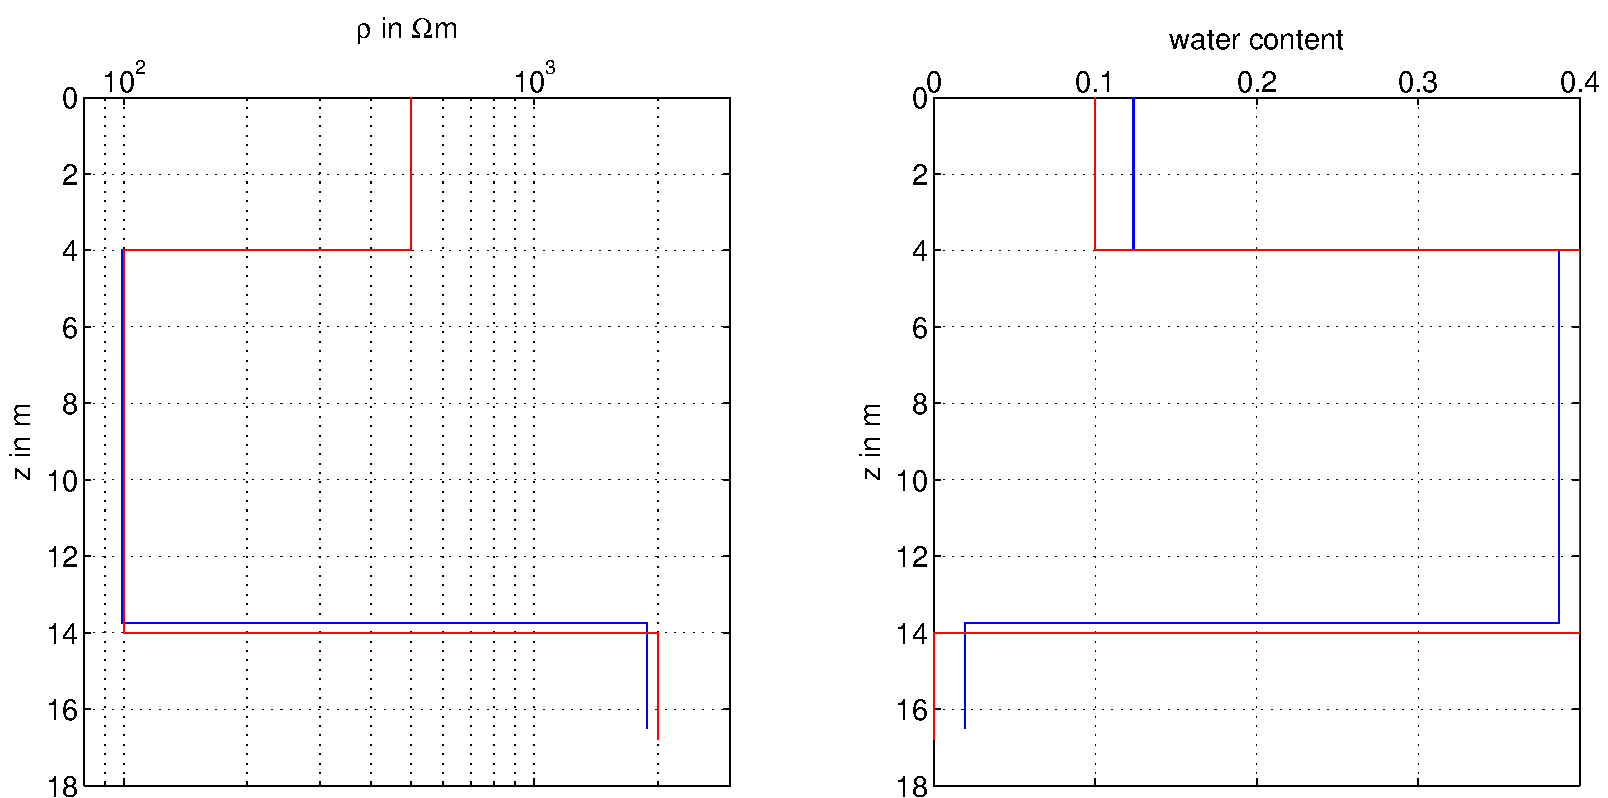
\includegraphics[width=0.9\textwidth]{dc_mrs_blockjoint}
\caption{Joint inversion result of block-coupled DC resistivity (left) and MRS (right) sounding.}\label{fig:blockjoint}
\end{figure}


%%%%%%%%%%%%%%%%%%%%%%%%%%%%%%%%%%%%%%%%%%%%%%%%%%%%%%%%%%%%%%%%%%%%%%%%%%%
\subsection{Structurally coupled cooperative inversion of DC and MRS soundings}\label{sec:structjoint}
File \file{doc/tutorial/code/joint/dc\_mrs\_joint1d.cpp}\\
In many cases it is not clear whether the model boundaries observed by different methods are identical or how many of them are existing.
Nevertheless we expect a similarity of the structure, i.e. the gradients.
On smooth model discretizations of any dimension the exchange of geometrical information can be achieved using the constraint control function \citep{guerue06nearsurface}.
Main idea is to decrease the weight for the roughness operator of one method depending on the partial derivative of the other.
A large roughness as a possible interface should enable the interface on the other side by a low weight.
There are different possible functions for doing so.
Originally, a iteratively re-weighted least squares scheme was proposed that incorporates the whole distribution.
Here we use a simple function
\begin{equation}
    w_c(r) = \frac{a}{|r|+a}+a
\end{equation}
where $w_c$ is the weight, $r$ is the roughness value and $a$ is a small quantity.
For $r\rightarrow 0$ the weight $w_c=1+a$ lies slightly above 1, for $r\rightarrow\infty$ it becomes $a$.

In this case we apply it to DC resistivity and MRS sounding for a smooth 1d model.
The latter operator is linear and thus realized by a simple matrix vector multiplication of the kernel function and the water content vector.
We initialise the two independent inversions and run one iteration step each.
In the iteration loop we calculate the function of one roughness and set it as constraint weight for the other before running another inversion step.
\begin{lstlisting}
    invMRS.setMaxIter( 1 );
    invDC.setMaxIter( 1 );
    invMRS.run(); //! init and run 1 step
    invDC.run(); //! init and run 1 step
    double a = 0.1;
    RVector cWeight( nlay - 1 );
    for ( int iter = 1; iter < maxIter; iter++ ) {
        cWeight = a / ( abs( invDC.roughness() ) + a ) + a;
        invMRS.setCWeight( cWeight );
        cWeight = a / ( abs( invMRS.roughness() ) + a ) + a;
        invDC.setCWeight( cWeight );
        invDC.oneStep();
        invMRS.oneStep();
    }
\end{lstlisting}

Figure \ref{fig:dcmrsstruct} shows the inversion result for the above mentioned three-layer case.
Without coupling (a) the transitions between the layers are quite smooth.
Much more significant jumps in both parameters occur when structural coupling is applied (b) and make the interpretation of both layer thickness and representative parameters less ambiguous.

\begin{figure}[htb]
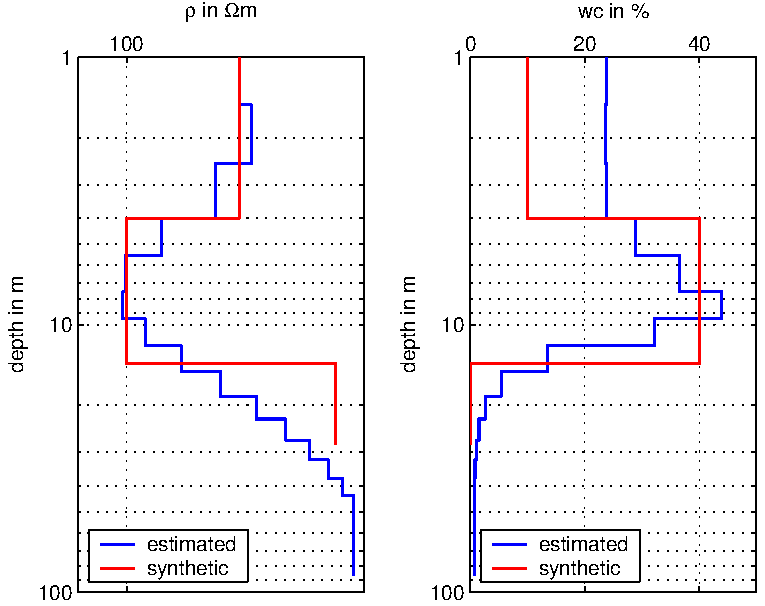
\includegraphics[width=0.5\textwidth]{DC-MRS-uncoupled}
\hfill
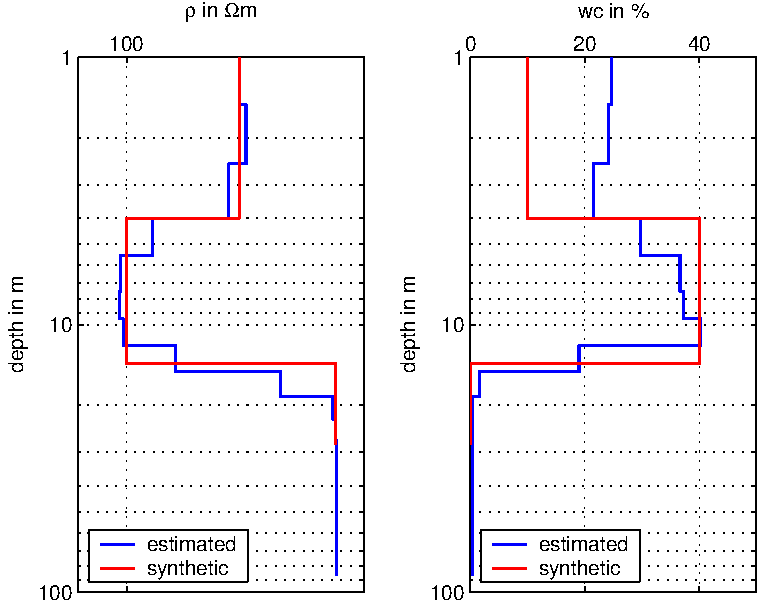
\includegraphics[width=0.5\textwidth]{DC-MRS-coupled}\\
\vskip -2ex 
a\hfill b%\\[1ex]
\caption{Synthetic model (red) and inversion results (blue) for DC (left) and MRS (right) 1D inversion without (a) and with (b) structural coupling}\label{fig:dcmrsstruct}
\end{figure} 

Of course the coupling does not have to affect the whole model.
The constraint weight vector can as well be set for an individual region such as the aquifer.
See inversion templates on how to do structural coupled inversion more easily and flexibly.

%%%%%%%%%%%%%%%%%%%%%%%%%%%%%%%%%%%%%%%%%%%%%%%%%%%%%%%%%%%%%%%%%%%%%%%%%%%
\subsection{Petrophysical joint inversion}\label{sec:petrojoint}
Target: water content in a soil column using GPR (CRIM equation) and DC (Archie equation)

\sperre{TO BE IMPLEMENTED}

\begin{figure}[htb]
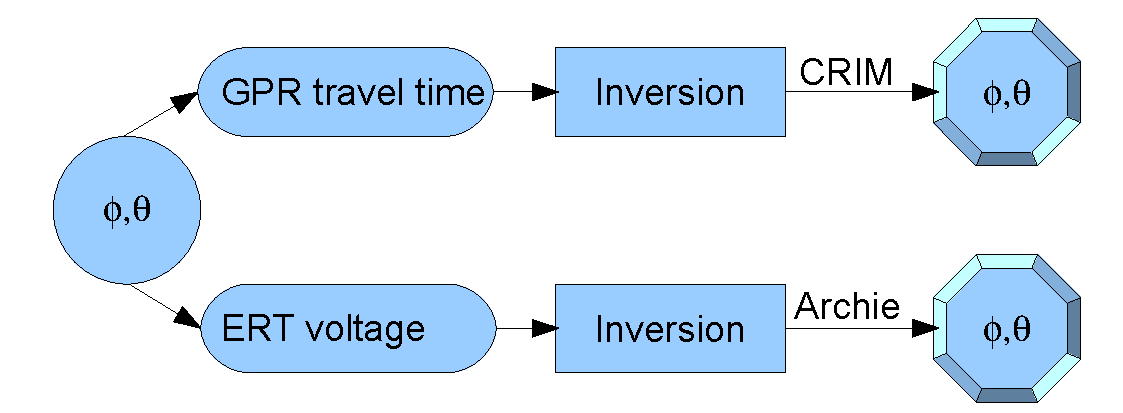
\includegraphics[width=0.5\textwidth]{petro1}
\hfill
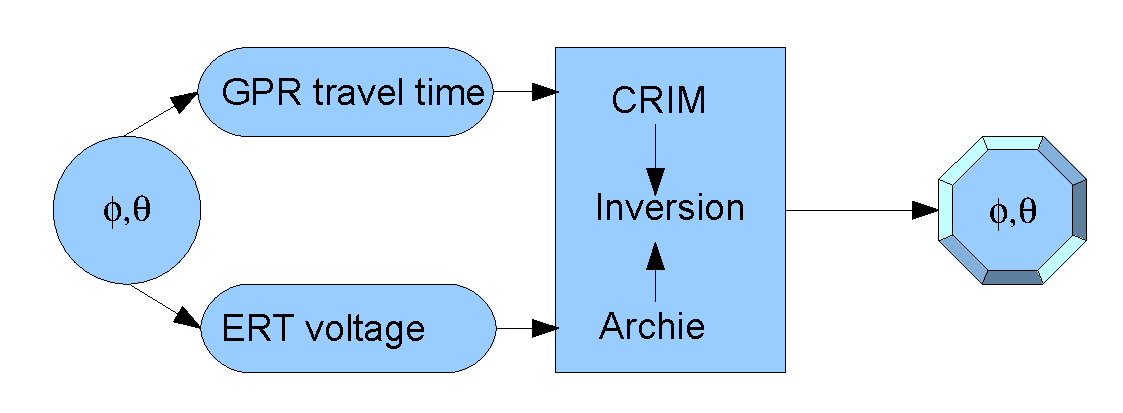
\includegraphics[width=0.5\textwidth]{petroji}\\
\vskip -8ex 
a\hfill b%\\[1ex]
\caption{Scheme for separate inversion (a) and petrophysical joint inversion (b) of GPR and ERT data to obtain an image of porosity or water content}\label{fig:petroji}
\end{figure} 
